\paragraph{Model-View-Controller}\cite{aspmvc}
This is an architectural template thta is used to separate responsibility of an application into three parts; the model, the view, and the controller.
A diagram, displaying the pattern and its internal dependencies, can be seen in \Cref{mvcdiagram}.

\begin{figure}[h]
\begin{center}
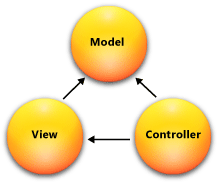
\includegraphics[width=0.5\textwidth]{mvc.pdf}
\caption{The MVC design pattern.}
\label{mvcdiagram}
\end{center}
\end{figure}

\begin{description}
\item [Model] contains the model of the application domain and takes care of fetching data from the underlying layers and making it available to the view and the controller.

\item [View] displays the model to the user.
In our case the view is the serialized resource representation, that the user obtains by performing requests against the API.
Per default, this is \texttt{text/xml}, however, by adding the \texttt{Accept} header\cite[Section 14]{http_specification}, this can be set to \texttt{application/json}.

\item [Controller] handles the interaction with users.
Based on user input, the controller works on the model and selects which view is needed to display the data.
\end{description}
